\newcommand{\specname}{BTSpec}
\newcommand{\status}{Beta}
\newcommand{\ecn}{NA}
\newcommand{\revdate}{2013-03-16}
\newcommand{\rev}{000}

\documentclass[dvips,12pt]{article}
\renewcommand{\contentsname}{3. Index} 

\usepackage{amsmath}
%\usepackage{program}
\usepackage{a4,color,graphics,palatino,fancyhdr}
\usepackage{lastpage}
\usepackage{fancyhdr}
\usepackage{changepage}% http://ctan.org/pkg/changepage
\usepackage{graphicx}
\usepackage{float}

\floatstyle{ruled}
\newfloat{program}{thp}{lop}
\floatname{program}{Source Code}


\setlength{\headheight}{15pt}

\setcounter{secnumdepth}{1}
\setcounter{tocdepth}{1}

\lhead{\specname}
\rhead{rev.\  \rev} 
\chead{\revdate}
\cfoot{\footnotesize Page\ \thepage\ of \pageref{LastPage}}
\pagestyle{fancy}
\title{BTspec}

\author{chaz}

\begin{document}

\frenchspacing


\section{Purpose}
Documentation for Simple Brewtroller Firmware

\tableofcontents
\listoffigures


\section{Objective}

\subsection{Goals}

The program aims to be a ``most simple'' firmware suitable for beer
brewing. It may also be useful for other temperature control applications
that need selectable open-loop control as well as closed-loop thermostatic control in the same unit.

\begin{figure}[h]
    \begin{centering}
    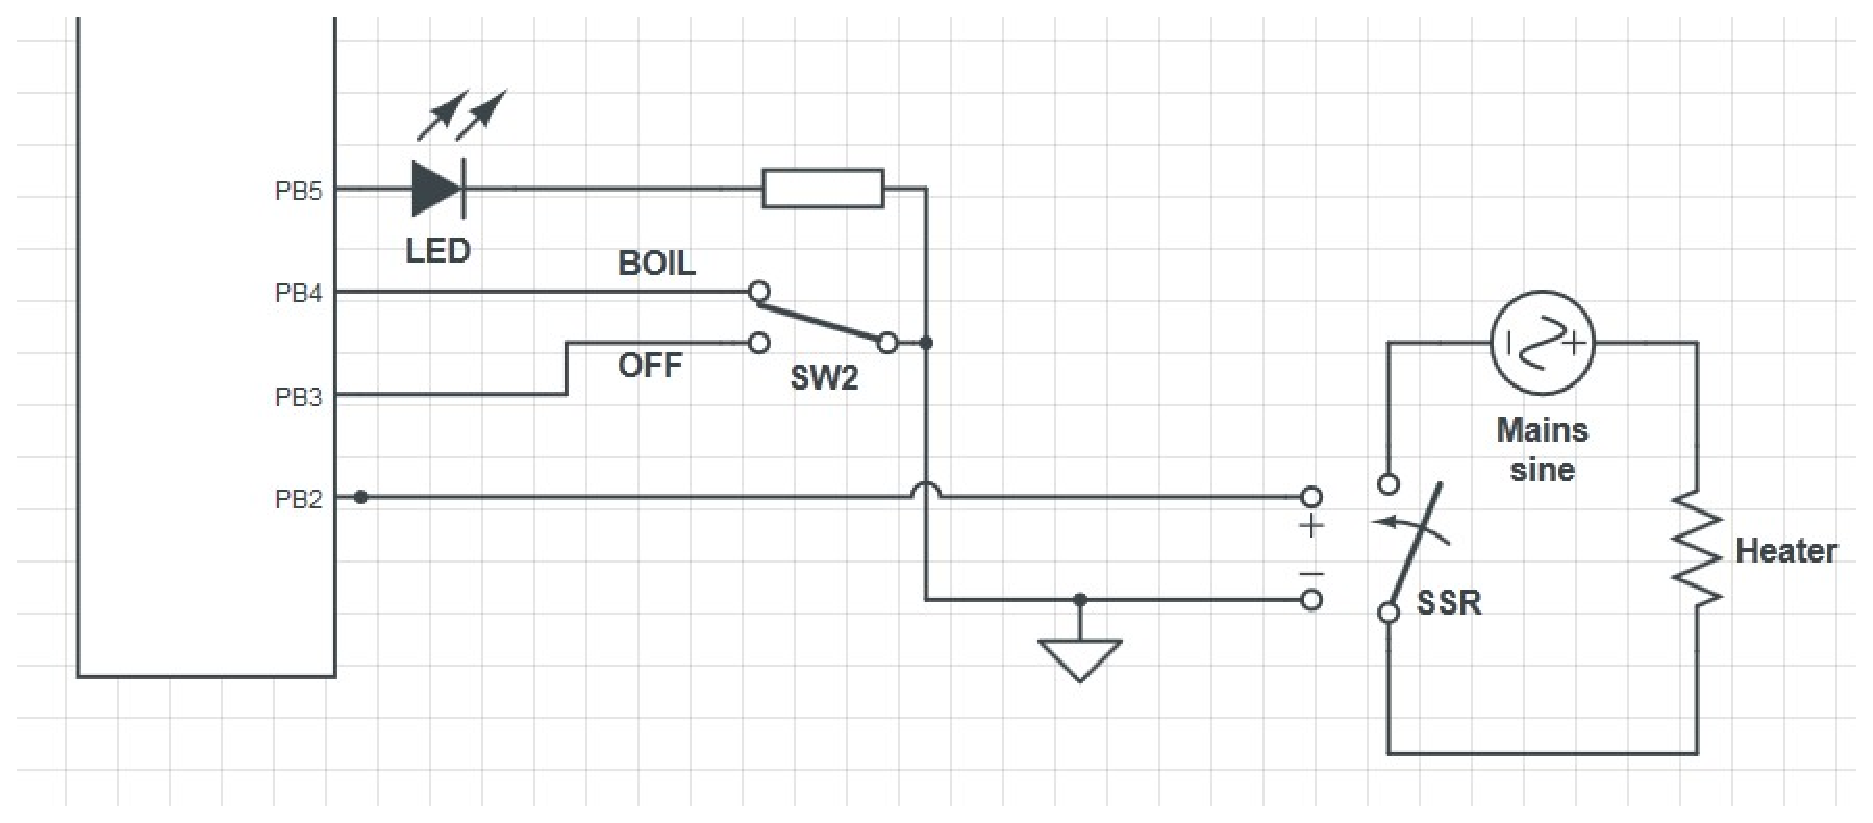
\includegraphics[width=0.8\textwidth]{min}
    \caption{Example Minimal System}
    \label{fig:min}
    \end{centering}
\end{figure}

\begin{figure}[h]
    \begin{centering}
    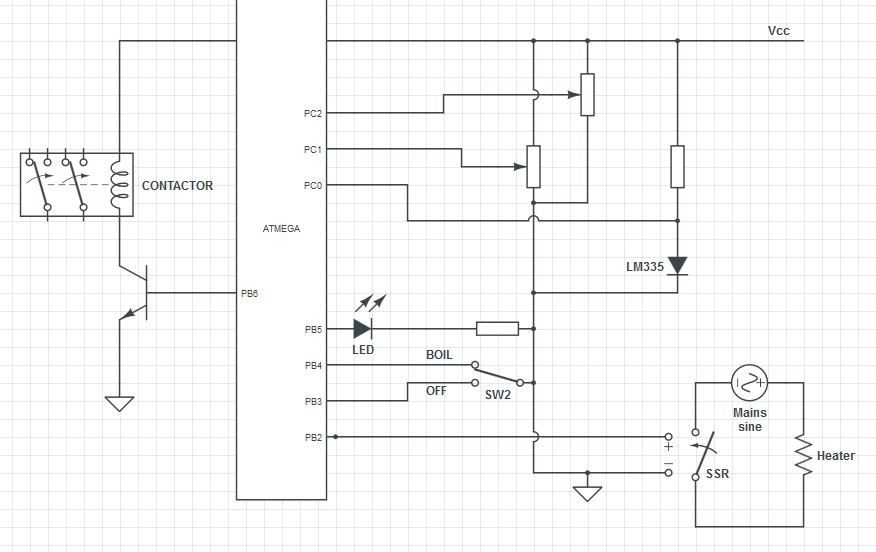
\includegraphics[width=0.8\textwidth]{max}
    \caption{Example Complete System with temp control, contactor and LED}
    \label{fig:max}
    \end{centering}
\end{figure}


\section{Microcontroller hardware}

The microcontroller used is an ATMEGA328 8-bit AVR\textcopyright\
microcontroller. It was selected for its availability. The firmware would
run on other AVR microcontrollers with minimal modification. The
microcontroller is powered by 5V and runs at 1MHz, which is how
it's configured out-of-the-box. No external crystal is needed, just apply
5V on the Vcc pin and pull up RESET. 

Flashing this firmware to the
microcontroller will require an in-system-programmer such as the AVRISPV2
or USBTinyISP. Instructions on programming AVR microcontrollers is outside
the scope of this document. All the cool kids are using Arduino nowadays,
and you may be able to pretend this is an Arduino program and try to flash
it with the Arduino IDE and it may Just Work. You are on your own on the Arduino
front.

\section{Perhipheral hardware options}

\renewcommand{\arraystretch}{1.4}% adjust hline heights for prettiness
\begin{figure}[h]
\centering
\begin{tabular}{|c|c|c|c|}
\hline
Input Item&AVR Pin&Voltage details& Function notes\\
\hline
Boil Switch&PB4&GND=ACTIVE&Set boil duty cycle \\
\hline
ON Switch&PB5&GND=OFF&kill SSR and contactor \\
\hline
Temp probe&PC0&0V-5V analog in&LM335 \\
\hline
BOIL pot&PC1&0V-5V analog in&Heating element power\\
\hline
TEMP pot&PC2&0V-5V analog in&Temp setpoint\\
\hline
\end{tabular}
\caption{Table Of Inputs}
\label{fig:inputs}
\end{figure}

\renewcommand{\arraystretch}{1.4}% adjust hline heights for prettiness
\begin{figure}[h]
\centering
\begin{tabular}{|c|c|c|c|}
\hline
Output Item&AVR Pin&Voltage details& Function notes\\
\hline
Blinkenled&PB2&LED+resistor&Blinks\\
\hline
SSR&PB5&Hook to SSR&5V=heater on\\
\hline
Contactor&PB5&for NO Contactor&5V=Contactor on\\
\hline
\end{tabular}
\caption{Table Of Outputs}
\label{fig:inputs}
\end{figure}

\section{Operating Details}

As you can see, the system is configurable. With nothing hooked up, the firmware does nothing. You can add
functionality by simply hooking up more hardware. For example, an output for a contactor
is provided, but if you leave it disconnected, no problem. An input for a
temp probe is provided, but if you leave it disconnected, the firmware just
ignores thermostat functionality. 

The simplest possible
hardware is a 2-position (or 3-position ``center-off'') switch connected to
the ``boil'' and ``off'' inputs. With a pull-up resistor on the ``BOIL''
pot input, this allows 3-way switching between ON, OFF, and BOIL. If you
want to control the boil with a knob, hook a pot up to the BOIL input. If
you want at thermostat, hook up a temp probe and another pot. 

A
full-featured system has a contactor, temp probe connection, 2 knobs, a 3-way, ``center-off'' switch to select ``OFF'',
``ON'', and ``BOIL''. When OFF, the contactor and SSR output are both off.
When ON, the contactor is on and the element is controlled thermostatically
whenever the temp probe is plugged in. 
The BOIL potentiometer is used to set the element 
duty cycle, whether or not a temp probe is connected. Placing the switch on
``BOIL'' fires the element at the pre-selected duty cycle for consistent
boiling.

\centering
\vspace{2cm}
\appendix

\end{document}

